%!TEX root = ../../main.tex
\chapter{Theoretische Grundlagen}
\section{Künstliche Intelligenz}
\ac{KI} wird zunehmend in verschiedenen Bereichen eingesetzt und erleichtert die Arbeit der Menschen enorm. Viele Arbeiten können mithilfe von \ac{KI} schneller und besser erledigt werden. Im nachfolgenden Abschnitt werden die Begriffe ``Intelligenz'' und ``Künstliche Intelligenz'' erklärt, um ein einfaches Verständnis dafür zu schaffen. Es werden außerdem die verwandten Begriffe Machine Learning und Deep Learning in den Kontext eingeordnet.

In der Psychologie bezieht sich Intelligenz auf die Fähigkeit logische, sprachliche, mathematische oder sinnliche Probleme zu lösen, es besteht jedoch keine allgemeine Definition darüber wie Intelligenz definiert ist. Der Mensch kann sich durch seine kognitiven Fähigkeiten, Beschreibungen oder Erklärungen von Sachen merken, welcher er zu einem späteren Zeitpunkt abrufen und verwenden kann. Das menschliche Gehirn, welches aus Milliarden von Neuronen besteht, lernt dabei gewisse Strukturen, Konzepte und Fähigkeiten kennen und speichert diese ab. Beim Lernen der Informationen werden Verbindungen zwischen den Neuronen im Gehirn gestärkt. Je öfter eine Sache gelernt wird, desto mehr stärken sich gewisse Verbindungen von Neuronen im Gehirn. \cite[vgl.][]{Ertel2021,Posthoff2022}

Die Künstliche Intelligenz hingegen, ist ein wissenschaftlicher Bereich, der sich damit befasst, den Computern das menschliche Verhalten anzueignen. Gemeint ist hierbei, dass ein Computer darauf trainiert wird in der Lage zu sein, ähnlich wie ein Menschen zu denken und darauf folgende Aktionen auszuführen. \cite[vgl.][]{Lang2023} Anders als bei biologischen Neuronen, lösen Computer Probleme wie die Klassifizierung eines Bildes durch die Anwendung von mathematischen Funktionen und Algorithmen. Man versucht die Fähigkeit des Denkens vom Menschen zu imitieren, um so einen Mehrwert bei Lösung von Problemen mit Computern zu bewirken. Mit Hilfe der künstlichen Intelligenz sind Computer heutzutage in der Lage Probleme zu lösen, die vorher ein höheres intellektuelles Verständnis erforderten. Computer können so bspw. Bilder klassifizieren oder auch Vorhersagen treffen. Ähnlich wie beim Menschen, lernen Computer durch verfügbare Daten und stärken dadurch bestimmte mathematische Verbindungen. \cite[vgl.][]{WasIstKi}


\begin{figure}[h]
	\centering
	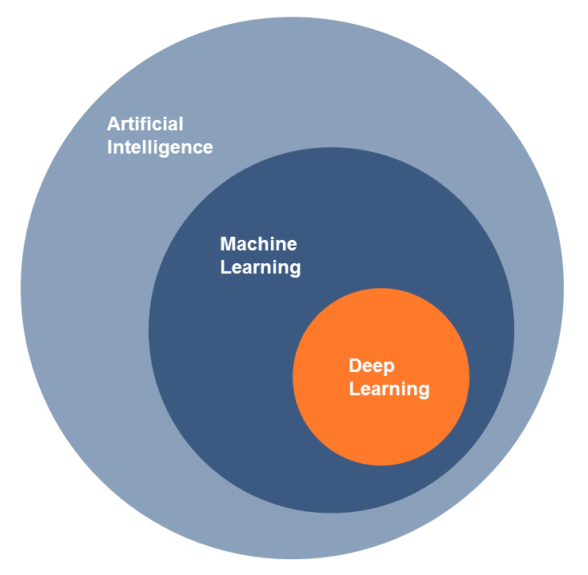
\includegraphics[height=.7\textwidth]{ai_overview.png}
	\caption{Übersicht der Bereiche von künstlicher Intelligenz (Quelle: \url{https://www.alexanderthamm.com/de/blog/ki_artificial-intelligence-ai-kuenstliche-neuronale-netze-machine-learning-deep-learning/})}
\end{figure}

Im Kontext der \ac{KI} ist oft auch die Rede von Machine Learning, Deep Learning und Neuronalen Netzen. \ac{KI} ist der Überbegriff, welcher sowohl Machine Learning als auch Deep Learning beinhaltet. Deep Learning ist eine Teilbereich des Machine Learnings, in welchem die künstlichen Neuronalen Netze zum Einsatz kommen, mit denen Computer in der Lage sind Dinge zu lernen und Probleme zu lösen. Nachfolgend liegt der Fokus auf dem Bereich des Deep Learnings.
